\ProvidesFile{seminar07.tex}

\section{Семинар 7}

\subsection{Задача 1}

\begin{enumerate}[label=\asbuk*)]

\item Сколько существует различных графов на данных $n$ вершинах?

\item Сколько существует различных ориентированных графов на данных $n$ вершинах?
\end{enumerate}

\subsubsection{Пункт А}
\begin{solution*}
Способов выбрать неупорядоченную пару вершин
\[
C^2_n = \frac{n(n-1)}{2}
\]
Для каждой неупорядоченной пары мы можем как проводить ребро, так и не проводить ребро. Тогда ясно, что графов на $n$ вершинах всего $2^{C^2_n}$ штук.
\end{solution*}

\subsubsection{Пункт Б}
\begin{solution*}
Способов выбрать упорядоченную пару вершин
\[
n(n-1)
\]
Для каждой упорядоченной пары мы можем как проводить ребро, так и не проводить ребро. Тогда ясно, что ориентированных графов на $n$ вершинах всего $ 2^{n(n-1)}$ штук.
\end{solution*}

\subsection{Задача 2}
Сколько существует различных попарно неизоморфных графов: а) на 4 вершинах; б)
на 5 вершинах?

\begin{solution*}
Едва-ли тут можно придумать что-то сильно лучше, чем перебор картинок.

\subsubsection{Пункт А}

\begin{figure}[H]
    \centering
    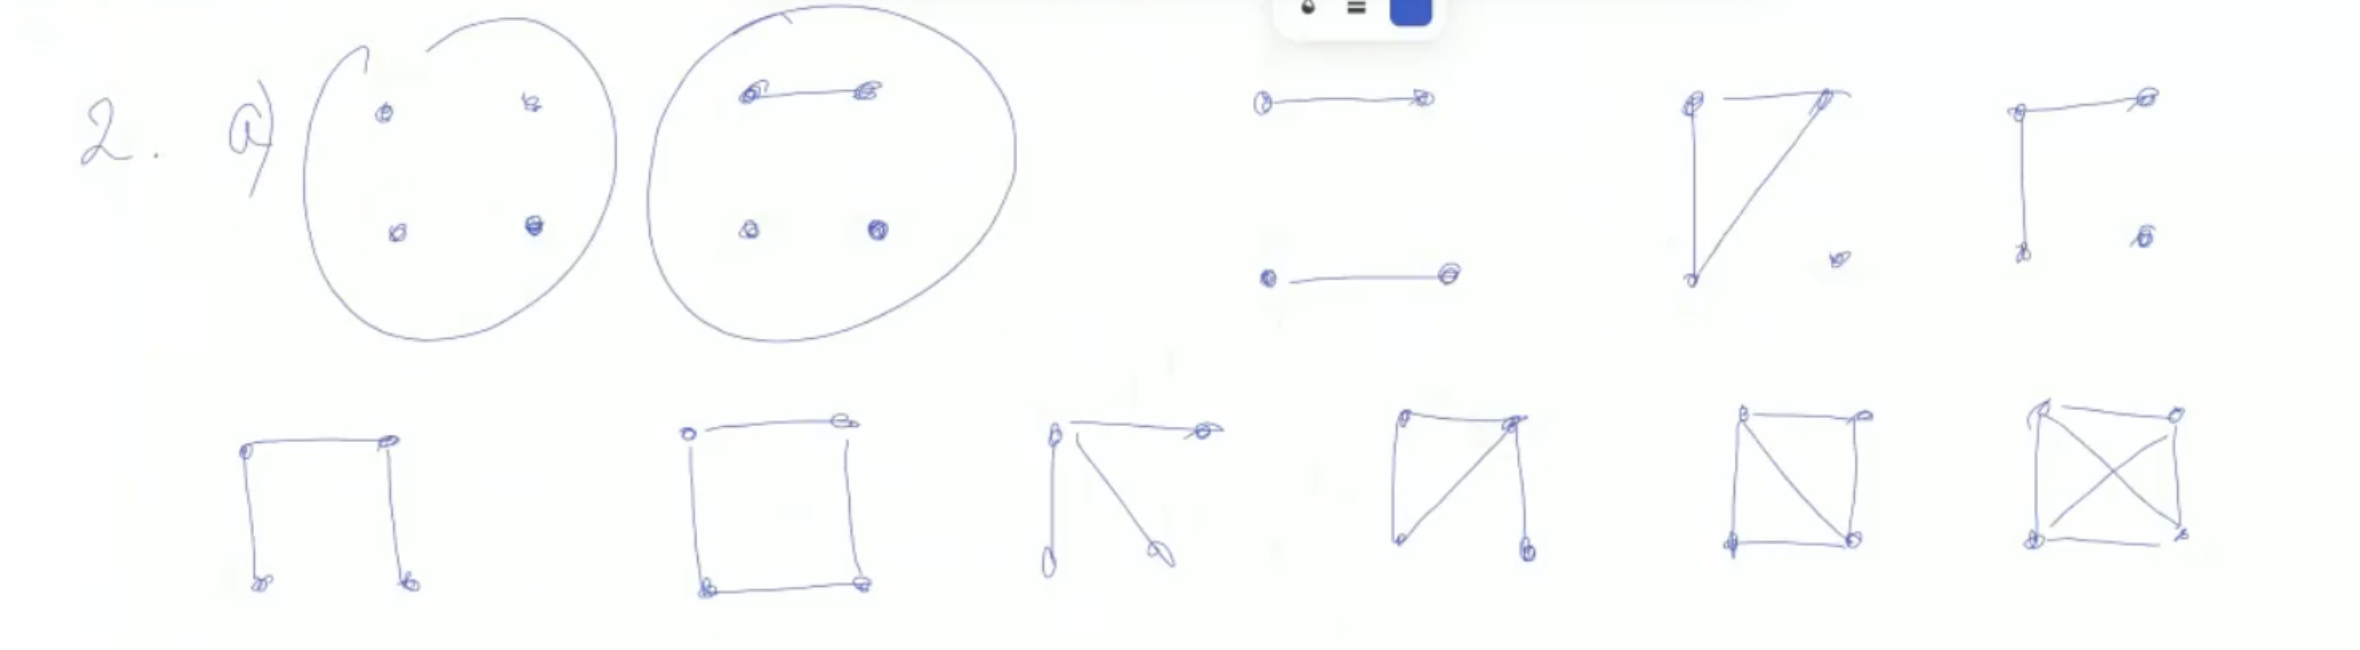
\includegraphics[width=1\linewidth]{Figures/sem08_task2.png}
\end{figure}

Ответ: 11

\subsubsection{Пункт Б}

Аналогично (гораздо больше картинок придется перебрать)\footnote{Вообще вопрос о том, сколько существует неизоморфных графов на $n$ вершинах, очевидно, изучен людьми менее кустарными методами. Результат для маленьких $n$ выписан \href{https://oeis.org/A000088}{тут} со ссылками на статьи}

Ответ: 34

\end{solution*}

\subsection{Задача 3}

Докажите, что в любом графе на $n \geq 2$ вершинах найдутся две вершины с одинаковой
степенью.

\begin{proof}
Ясно, что возможные степени вершин в графе на $n$ вершинах -- это $0, 1, \ldots, n - 1$.

При этом 0 и $n-1$ не могут присутствовать одновременно. То есть всего имеется $n-1$ доступный вариант степени для $n$ вершин. Тогда по принципу Дирихле найдутся две вершины одинаковой степени
\end{proof}

\subsection{Задача 4}

\begin{enumerate}[label=\asbuk*)]
    \item Докажите, что если между двумя вершинами в графе есть путь, то между ними есть и простой путь.
    \item Докажите, что если в графе есть цикл, то есть и простой цикл.
\end{enumerate}

\subsubsection{Пункт А}

\begin{proof}
Неформально: выкидываем <<ненужные>> участки пути из пути и победа.

Чуть более формально: пусть у нас есть путь 
\[
v_0, e_1, v_1, \ldots e_k, v_k
\]

Если в нём нет одинаковых вершин, то и доказывать нечего.

Если же в нём есть одинаковые вершины, то рассмотрим первое вхождение в эту вершину и последнее вхождение в эту вершину. Например, для вершины $v_i$:
\[
v_0, e_1, v_1, \ldots, \underbrace{v_i, e_{i+1}, \ldots,}_{\text{эту часть можно выкинуть}} v_i, \ldots, e_k, v_k\textbf{}
\]
Выкидываем из пути выделенную часть. Делаем так до тех пор, пока путь не станет простым. Ясно, что этот алгоритм остановится, так как граф на конечном числе вершин.

\subsubsection{Пункт Б}
Абсолютно аналогично пункту А. Нужно лишь заменить слово <<путь>> на слово <<цикл>>.
\end{proof}

\subsection{Задача 5}
У Пети всего 28 одноклассников. У каждых двух из 28 различное число друзей в этом классе. Сколько друзей у Пети?\footnote{На всякий случай уточню, что имеется в виду, что всего людей 29 (Петя и ещё 28 одноклассников)}
\begin{solution*}
Ясно, что в графе на 29 вершинах степень каждой вершины может быть одним из чисел $0, 1, \ldots, 28$.

Предположим, что среди 28 одноклассников Пети есть степень вершины 0. В таком случае в графе нет степени вершины 28. Значит, из-за того, что у одноклассников попарно разное число друзей в классе, степени вершин у 28 одноклассников Пети в точности равны $0, 1, \ldots, 27$.

С другой стороны, если же степени вершины 0 среди 28 одноклассников Пети нет, то по безысходности у 28 одноклассников Пети степени вершин в точности равны $1, 2, \ldots, 28$.

Два случая разбираются абсолютно аналогично.

\begin{figure}[H]
    \centering
    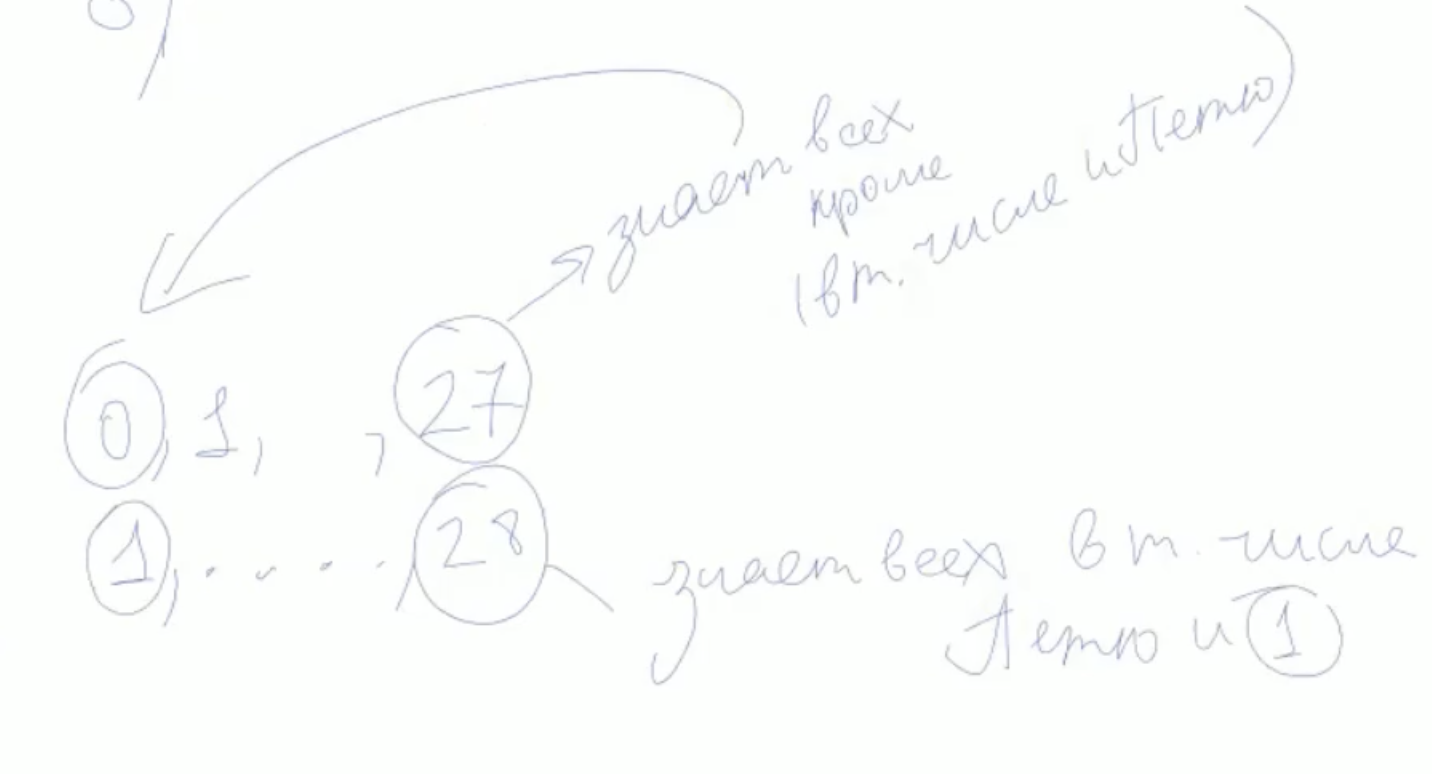
\includegraphics[width=0.75\linewidth]{Figures/sem08_task5.png}
\end{figure}

Смотрите: в первом случае у нас есть человек со степенью вершины 0 и человек со степенью вершины 27. Ясно, что первый человек не дружит ни с кем. А второй дружит со всеми, кроме нуля. Ну значит, он дружит и с Петей.

Во втором случае у нас человек со степенью вершины 28. Ясно, что первый человек дружит только со вторым, а второй человек дружит вообще со всеми. Ну значит, он дружит и с Петей.

Теперь финт ушами. На этом шаге мы в любом из двух случаев поняли, что у Пети есть +1 друг.

Давайте отщипнем в обоих случаях первого и второго человека (то есть того, кто дружит с наименьшим числом людей и того, кто дружит с наибольшим числом людей). И будем рассматривать граф без них.

Тогда степень оставшихся людей уменьшиться ровно на 1. Действительно: они точно дружили со вторым (тот, который дружил с наибольшим числом людей) и точно не дружили с первым (тот, который дружил с наименьшим числом людей). 

Последовательно будем применять к оставшимся графам подобное рассуждение. Тогда ясно, что у Пети 14 друзей.

\textbf{Ответ:} 14

\subsection{Задача 6}

Докажите, что среди любых 6 людей найдутся или трое попарно знакомых, или трое
попарно незнакомых.

\begin{proof}
Рассмотрим произвольного человека.

Ясно, что у него есть либо хотя бы 3 знакомых, либо хотя бы 3 незнакомых среди оставшихся.

Рассмотрим первый случай (второй разбирается симметрично). 

\begin{figure}[H]
    \centering
    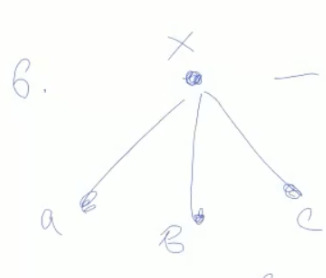
\includegraphics[width=0.5\linewidth]{Figures/sem08_task6.png}
\end{figure}

Если среди 3 его знакомых есть хотя бы одна пара знакомых, то вот мы и получили тройку знакомых.

А если нет -- то мы получили тройку незнакомых.
\end{proof}


\end{solution*}